\documentclass[12pt, twoside]{report}

\usepackage[a4paper, margin=1.5cm]{geometry}
\usepackage{xcolor}

\usepackage{minted}
\definecolor{bg}{rgb}{0.95,0.95,0.95}
\setminted[python]{
    autogobble=true,
    linenos=true,
    numbers=left,
    python3=true,
    xleftmargin=0.75cm,
    xrightmargin=0.75cm,
    bgcolor=bg,
    fontsize=\small
}
\setmintedinline[python]{
    bgcolor={}
}
\usepackage{etoolbox}
%\BeforeBeginEnvironment{minted}{\vspace{0cm}}
%\AfterEndEnvironment{minted}{\vspace{-2cm}}

\BeforeBeginEnvironment{minted}{\vspace{0cm}}
\AfterEndEnvironment{minted}{\vspace{-0.75cm}}

%\BeforeBeginEnvironment{listing}{\vspace{0cm}}
%\AfterEndEnvironment{listing}{\vspace{0cm}}

\usemintedstyle{xcode} 

\usepackage{titlesec}
\titlespacing*{\chapter}{0pt}{-20pt}{16pt}
\titleformat{\chapter }[display]{\normalfont\Large\bfseries}{\chaptertitlename\
\thechapter}{10pt}{\Huge}

\usepackage{graphicx}
\usepackage{hyperref}

\usepackage{amsmath}
\usepackage{amssymb}
\usepackage{amsthm}

\usepackage{enumitem}
\usepackage{siunitx}

\theoremstyle{plain}
\newtheorem{theorem}{Theorem}[chapter]
\theoremstyle{definition}
\newtheorem{definition}{Definition}[chapter]
\newtheorem{corollary}{Corollary}[theorem]
\theoremstyle{definition}
\newtheorem{example}{Example}[chapter]

\providecommand{\abs}[1]{\lvert#1\rvert}
\providecommand{\norm}[1]{\lVert#1\rVert}

\begin{document}


% The 'article' document class provides a simple way to make a title
% page: 

\title{
    \large{Numerical Solution to the Initial Value Problem by a 
    Predictor-Corrector Method:}\\
    Applications to n-Body Problem and Pendula}
\author{Joel Biffin}
\maketitle

% A table of contents can be generated automatically as well:

\tableofcontents


\begin{abstract}

    Initial Value Problems primarily arise from the modelling of natural
    phenomena where often we are able to desribe some quantity's rate of change
    as a function of itself coupled with time. This report will focus on
    Initial Value Problems arising from models using Ordinary Differential
    Equations. It is notable that many of the breakthroughs in the field of
    solving Partial Differential Equations have arisen from spacially
    discretising the problem and approximating solutions to the discretised
    Initial Value Problem.

    Leibniz and Newton are often cited as the fathers of the field of
    differential equations. Similar to Newton, in this report we will be
    considering quantities which change with respect to time, but all of the
    methods and analyses apply for any other variable too. 

    Until the late 19th century, numerical algorithms to approximate solutions
    to Initial Value Problems could not usefully be applied. Since then
    contributions from Adams, Milne, Butcher and Gear (to name a few) have been
    used in computations an unimaginable number of times as a result of now 
    readily available computing power. 

    In this report, established methods will be analysed and reviewed 
    comparatively in terms of implementation complexity, computational cost
    and accuracy.

\end{abstract}


% Now comes the true content. 

\chapter{Background}
    
    \section{Notation}
    \label{1_notation}
        Throughout this report, vector quantities and functions will be written
        in lowercase bold type ($\mathbf{u}, \mathbf{f}$), scalar quantities 
        and functions will be written in lowercase type ($t, f$), and iterative
        schemes will use subscripting to represent the $i$-th iteration 
        ($u_{i}, \mathbf{u}_i$) of a method. Generally, vector quantities will
        be expressed as such rather than element-wise, unless otherwise stated.

        Chapter 3 gives reference to \textit{solvers}--this italicised  


    \section{Initial Value Problems}
    \label{1_ivp}
        An Initial Value Problem (IVP) can generally be written in the form,
        \begin{equation}
        \label{eq:ivp}
            \begin{split}
                \frac{d \mathbf{u}(t)}{dt}& = \mathbf{f}(t, \mathbf{u}), 
                \quad t \in [a, b]\\
                \mathbf{u}(a)& = \mathbf{u}_0, \quad \text{(given)},
            \end{split}
        \end{equation}
        using vector quantities. It is worth noting that this is in the form of
        a 1st order system of differential equations, this is due to the fact 
        we can reduce any $n$-th order equation to a system of first order ones
        (see section ).


    \section{Where Do They Come From?}
    \label{1_origins}
        As discussed in the abstract, IVPs often arise from, but are not
        restricted to, the modelling of natural phenomena. 

        Newton's 2nd Law of Motion describes the proportionality of the rate 
        of change of velocity to the resultant force acting on a body. This 
        coupled with an initial condition $\mathbf{v}(a)=\mathbf{v}_0$, gives
        an IVP. In electrical circuit modelling, the flow of charge $q$ from a
        capacitor of known initial charge $q(0)=q_0$ can too be modelled by an 
        IVP in the form of \eqref{eq:ivp}.


    \section{Existence \& Uniqueness of Solutions}
    \label{1_existence}
        Before discussing methods used to approximate solutions to IVPs, it is
        important to ascertain whether solutions do in fact exist and, if so,
        whether or not they are unique. We will use Lipschitz continuity to do
        so.
        \begin{theorem}
        \label{1_existence_uniqueness}
            Let $f(t,u)$ be a continuous function for all $u$ and $t \in 
            [a, b]$, and suppose that $f$ satisfies the Lipschitz condition,
            \begin{equation}
            \label{eq:lipschitz}
                \abs{f(t,v)-f(t,w)} \le L\abs{v-w},
                \quad \forall v, w \text{ and } t \in [a,b].
            \end{equation}
            Then, for any $u_0$ there exists a unique continuously
            differentiable function $u(t)$ defined on $[a,b]$ satisfying
            \eqref{eq:ivp}.
        \end{theorem}
        This result is incredibly important when modelling environments and 
        phenomena. If a model equation does not satisfy our Lipschitz condition
        this is a real indicator of whether or not our model correctly 
        represents our system.

        For the remainder of this report we will be concerned with problems 
        which do satisfy our Lipschitz condition \eqref{eq:lipschitz}.


    \section{Analytical Methods vs Numerical Methods}
    \label{1_analytical_numerical}
        Analytical methods can be used to solve IVPs but only for a very limited
        number of special cases. In terms of computing, there are a number of 
        software packages that are able to solve these differential equations
        symbolically (for example, MATLAB's `MuPAD'). Since it is the case that
        the majority of ordinary differential equations cannot by solved 
        analytically, these algorithms are of little use (and it's worth noting
        that these algorithms are notoriously costly).

        This inability to analytically find solutions led to the discussion of
        numerical methods to approximate solutions to IVPs at a specific $t$. 
        The general approach for these numerical methods begins with 
        discretising our independent variable $t$ into a mesh. This mesh is an 
        increasing monotonic sequence of time values ${\lbrace 
        t_i\rbrace}_{i=0}^n$, where $[a,b]$ has been split into $n$ (not 
        necessarily equally spaced) intervals such that $a=t_0$ and $b=t_n$.

        In practice, numerical methods are the best approach to finding 
        solutions to IVPs and when used appropriately they produce incredibly 
        useful results to equations that we would otherwise be unable to solve.

        In the next chapter we will be discussing what it is that makes a 
        numerical algorithm appropriate for a given problem. We will also be
        investigating the accuracy of our approximations.



\chapter{Numerical Methods}
\label{2_methods}
    Algorithms which approximate solutions to \eqref{eq:ivp} fall into three
    categories: Taylor Series methods, Linear Multistep Methods (LMMs) and 
    Runge-Kutta methods. It can be viewed that all three of these families are
    generalisations of Euler's Method (\ref{2_forward_euler}). 

    The focus of this project primarily lies with Linear Multistep Methods and 
    using them in the form of a predictor-corrector pair. Runge-Kutta methods
    are too used and evaluated here, but are only featured in case studies
    as starting schemes for LMMs.

    For the purposes of software design we have classified Euler's Method as a
    One-Step method, and similarly Runge-Kutta methods are classified as 
    One-Step methods too. Unless explicitly stated, all methods will use a 
    fixed step-size $h=\frac{b-a}{n}$ (where $n$ is the number of time 
    intervals) producing an equally spaced mesh.

    \section{One-Step Methods}
    \label{2_onestep}
        
        \subsection{(Forward) Euler's Method}
        \label{2_forward_euler}
            Euler's method is given by the iterative scheme,
            \begin{equation}
            \label{eq:euler}
                \mathbf{u}_{i+1} = \mathbf{u}_i + h\mathbf{f}(t_i, 
                \mathbf{u}_i).
            \end{equation}
            This scheme is \textit{explicit} since we can calculate 
            $\mathbf{u}_{i+1}$ using a combination of $\mathbf{u}_i$ and $t_i$
            which are known at the start of an iteration.

            \begin{definition}
                An iterative scheme is called \textbf{explicit} if at the 
                beginning of an iteration we can express $\mathbf{u}_{i+1}$ in 
                terms of values which have already been computed or can be 
                computed by simple substitution during the iteration. In 
                contrast, \textbf{implicit} schemes have $\mathbf{u}_{i+1}$ 
                appearing on both `sides' of our scheme, so an algebraic 
                equation must be solved at each iteration to compute 
                $\mathbf{u}_{i+1}$.
            \end{definition}

            We will discuss later on how the explicit nature of a method 
            impacts its stability.

        \subsection{(Backward) Euler's Method}
        \label{2_backward_euler}
            This method can be viewed as an \textit{implicit} variant of 
            \eqref{eq:euler}, and is given by
            \begin{equation}
            \label{eq:backward_euler}
                \mathbf{u}_{i+1} = \mathbf{u}_i + h\mathbf{f}(t_{i+1}, 
                \mathbf{u}_{i+1}).
            \end{equation} 
            Since $\mathbf{u}_{i+1}$ appears on both sides of our expression,
            we must solve
            \begin{equation}
            \label{eq:nonlinear_equation}
                \mathbf{g}(\mathbf{u}_{i+1}) = \mathbf{u}_{i+1} - 
                \mathbf{u}_i - h\mathbf{f}(t_{i+1}, \mathbf{u}_{i+1}) 
                = \mathbf{0}
            \end{equation}
            for $\mathbf{u}_{i+1}$ at every iteration.

            Of course, we could solve this symbolically at a cost, but in
            practice we use any numerical (vector) root finding algorithm 
            (Secant Method, Newton's Method etc.). 

            Originally in this project Newton's Method was applied using the 
            \mintinline{python}{scipy.optimize.newton} package in Python where 
            the Jacobian matrix was approximated via Finite Differences. As is 
            conventional, the initial `guess' solution was computed via 
            \eqref{eq:euler}. Unfortunately this method led to some 
            non-convergent solutions being returned. Eventually the decision 
            was made to use the \mintinline{python}{scipy.optimize.fsolve} 
            package which implements a variant of the Powell hybrid method.


    \section{Global \& Local Truncation Error}
    \label{2_error}
        As with any numerical approximations, our methods will introduce 
        errors. Here we will include floating point errors in our
        truncation error considerations, so floating point errors are not
        noted directly but are considered in implementation.

        \begin{definition}
            The \textbf{Global Truncation Error} (GTE), denoted $e_{i}(t)$,
            is the total error in our approximation. It is given by 
            $e_i=u(t_i) - u_i$, where $i$ represents the $i$-th iteration
            in the standard way (see Subsection \ref{1_notation}).
        \end{definition}

        \begin{definition}
            The \textbf{Local Truncation Error} (LTE), denoted $\tau (h)$,
            for a numerical method is the error introduced in one single 
            iteration. This is the error introduced in computing 
            $\mathbf{u}_{i+1}$ when all previously computed values are taken 
            to be exact.
        \end{definition}

        GTE is really just a consequence of LTE and due to this it is helpful
        to address our full attention to the analysis of LTE.
        
        For any method we can derive an expression for the order of LTE by 
        using a Taylor Series expansion for the exact solution to the ODE and
        take the difference between that and our iterative scheme (when all 
        previous values are taken to be exact). Doing this for Euler's method 
        is shown:
        
        Suppose $u_i = u(t_i)$, then Euler's method gives us, 
        \begin{equation}
            \begin{split}
                u_{i+1} &= u(t_i) + hf(t_i, u(t_i)) \\
                &= u(t_i) + hu'(t_i),\quad
                \text{since } u'(t_i) = f(t_i, u(t_i)).
            \end{split}
        \end{equation}
        Our Taylor expansion for our exact solution is,
        \begin{equation}
            u(t_{i+1}) = u(t_i + h) = u(t_i) + hu'(t_i) + \frac{h^2}{2} 
            u''(\xi_i) + O(h^3), \quad \xi_i \in (t_i, t_{i+1}).
        \end{equation}
        Taking the difference of these two expressions leaves us the remainder,
        \begin{equation}
            \tau(h) = u(t_{i+1}) - u_{i+1} = \frac{h^2}{2} u''(\xi_i) + 
            O(h^3) = O(h^2),
        \end{equation}
        so we know that for Forward Euler we have $\tau(h)=O(h^2)$.

        It's worth noting that a similar process can be carried out to find an expression for GTE but without the assumption that 
        $u_i=u(t_i)$. 
        \begin{definition}
            A method is said to be of \textbf{order} $p$ if its LTE satisfies 
            $\tau(h)=O(h^{p+1})$. If $p \ge 1$ then we say that the method is
            consistent of order $p$.
        \end{definition}
        With this definition we know that Forward Euler is an order 1 method 
        -- so too is Backward Euler. In addition, when our method is order $p$,
        we know that the GTE, $e_i=O(h^p)$ too.


    \section{Convergence \& Stability}
    \label{2_stability}
        Efforts in using these numerical algorithms would be fruitless if the 
        results obtained were not representative of the \textit{true} solution.
        So it is important that we know a method is \textit{convergent} before 
        using it.

        \begin{definition}
            A method is said to be \textbf{0-stable} if a small perturbation 
            $\boldsymbol{\varepsilon}$ ($\norm{\boldsymbol{\varepsilon}} 
            << 1$) to $\mathbf{u}_0$ causes the numerical solution to change 
            at most by $K\boldsymbol{\varepsilon}$, where $K$ is independent 
            of $h$.
        \end{definition}

        We will later discuss the \textit{root condition} which can be used as
        a quantitative method to establish 0-stability, but for the moment this
        qualitative definition is all we need.

        \begin{theorem}[Dahlquist's Equivalence Theorem]
        \label{2_dahlquist}
            A numerical method is said to be convergent of order $p$ if and 
            only if it is 0-stable and consistent of order $p$.
        \end{theorem}

        \begin{corollary}
        \label{2_dahlquist_corollary}
            A convergent numerical method has the property that,
            \begin{equation}
                \lim_{h \to 0} \norm{\mathbf{u}(t_i) - \mathbf{u}_i} = 0.
            \end{equation}
        \end{corollary}

        In practice, we are computing with floating point numbers so, in an 
        arbitrary precision, by taking $h$ to be excessively small then the 
        accuracy that we might theoretically gain will be counteracted by round-off errors.
        

        \subsection{Absolute Stability}
        \label{2_absolute_stability}
            Given that a method is \textit{0-stable} we know that if we take 
            $h$ to be sufficiently small we acheive a very good representation
            of the true solution. But how small does $h$ have to be? Are there any limitations on how \textit{large} $h$ is?

            Consider the scalar \textit{test equation},
            \begin{equation}
            \label{2_test_equation}
                u' = \lambda u, \quad \lambda \in \mathbb{C},
            \end{equation}
            whose solution is known, $u(t)=c e^{\lambda t}$ for some constant 
            $c$. When $\mathbb{R}\text{e}\{\lambda\} < 0$, our solution 
            converges to 0 as $t\to\infty$. This results in the absolutely 
            decreasing sequence of approximations 
            ${\lbrace u_i \rbrace}_{i=0}^{\infty}$.

            We want our numerical methods to share this property when acting 
            on the test equation.

            \begin{definition}
                The \textbf{region of absolute stability} is the set of 
                $h\lambda\in\mathbb{C}$ where 
                ${\lbrace u_i \rbrace}_{i=0}^{\infty}$ is an absolutely
                decreasing sequence.
            \end{definition}

            We can find the region of absolute stability by applying our 
            numerical method to the test equation. For forward Euler we attain 
            the region $\abs{1+h\lambda} \le 1$ which provides us a very 
            restrictive upper bound on the value of $h$ we can choose. 
            Applying backward Euler gives the region 
            $\abs{1-h\lambda}^{-1} \le 1$, which is satisfied for all values 
            of $h, \lambda$ where $\mathbb{R}\text{e}\{\lambda\} \le 0$.
            Hence the entire left half-plane is in the region of stability and 
            there is no restriction on the value of $h$ we can choose.

            \begin{definition}
                A numerical method having the full left-half plane in its 
                region of absolute stability is said to be \textbf{A-stable}.
            \end{definition} 


        \subsection{Stiffness}
        \label{2_stiffness}
            Ideally we would be able to choose our step size $h$ based solely
            on the accuracy we want from our computation. Unfortunately this is
            not always the case -- as highlighted by our region of absolute
            stability for forward Euler. The \textit{stiffness} of a system
            helps to characterise this problem.

            \begin{definition}
                An IVP is said to be \textbf{stiff} if the step size required 
                to satisfy our absolute stability requirement is significantly
                smaller than the step size required to approximate at some 
                desired accuracy.
            \end{definition}

            \begin{example}
                Consider the IVP,
                \begin{equation}
                \label{eq:2_stiff_ex}
                    \begin{cases}
                        u'(t) = 100u(t), \quad \text{on } t \in [0,0.2],\\
                        u(0) = 10.
                    \end{cases}
                \end{equation}
                Figure \ref{2_stiff_graphs} demonstrates the impact of our 
                equation's stiffness on our results using forward Euler. By 
                method of substitution, our absolute stability expression 
                tells us that in order to compute stable approximations using 
                \eqref{eq:euler} we must use $h \le 0.02$. In contrast, we 
                have no bound on our choice of $h$ in terms of stability for 
                backward Euler. This is highlighted by the general shape of 
                our graphs in comparison to results from forward Euler.

                \begin{figure}
                    \centering
                        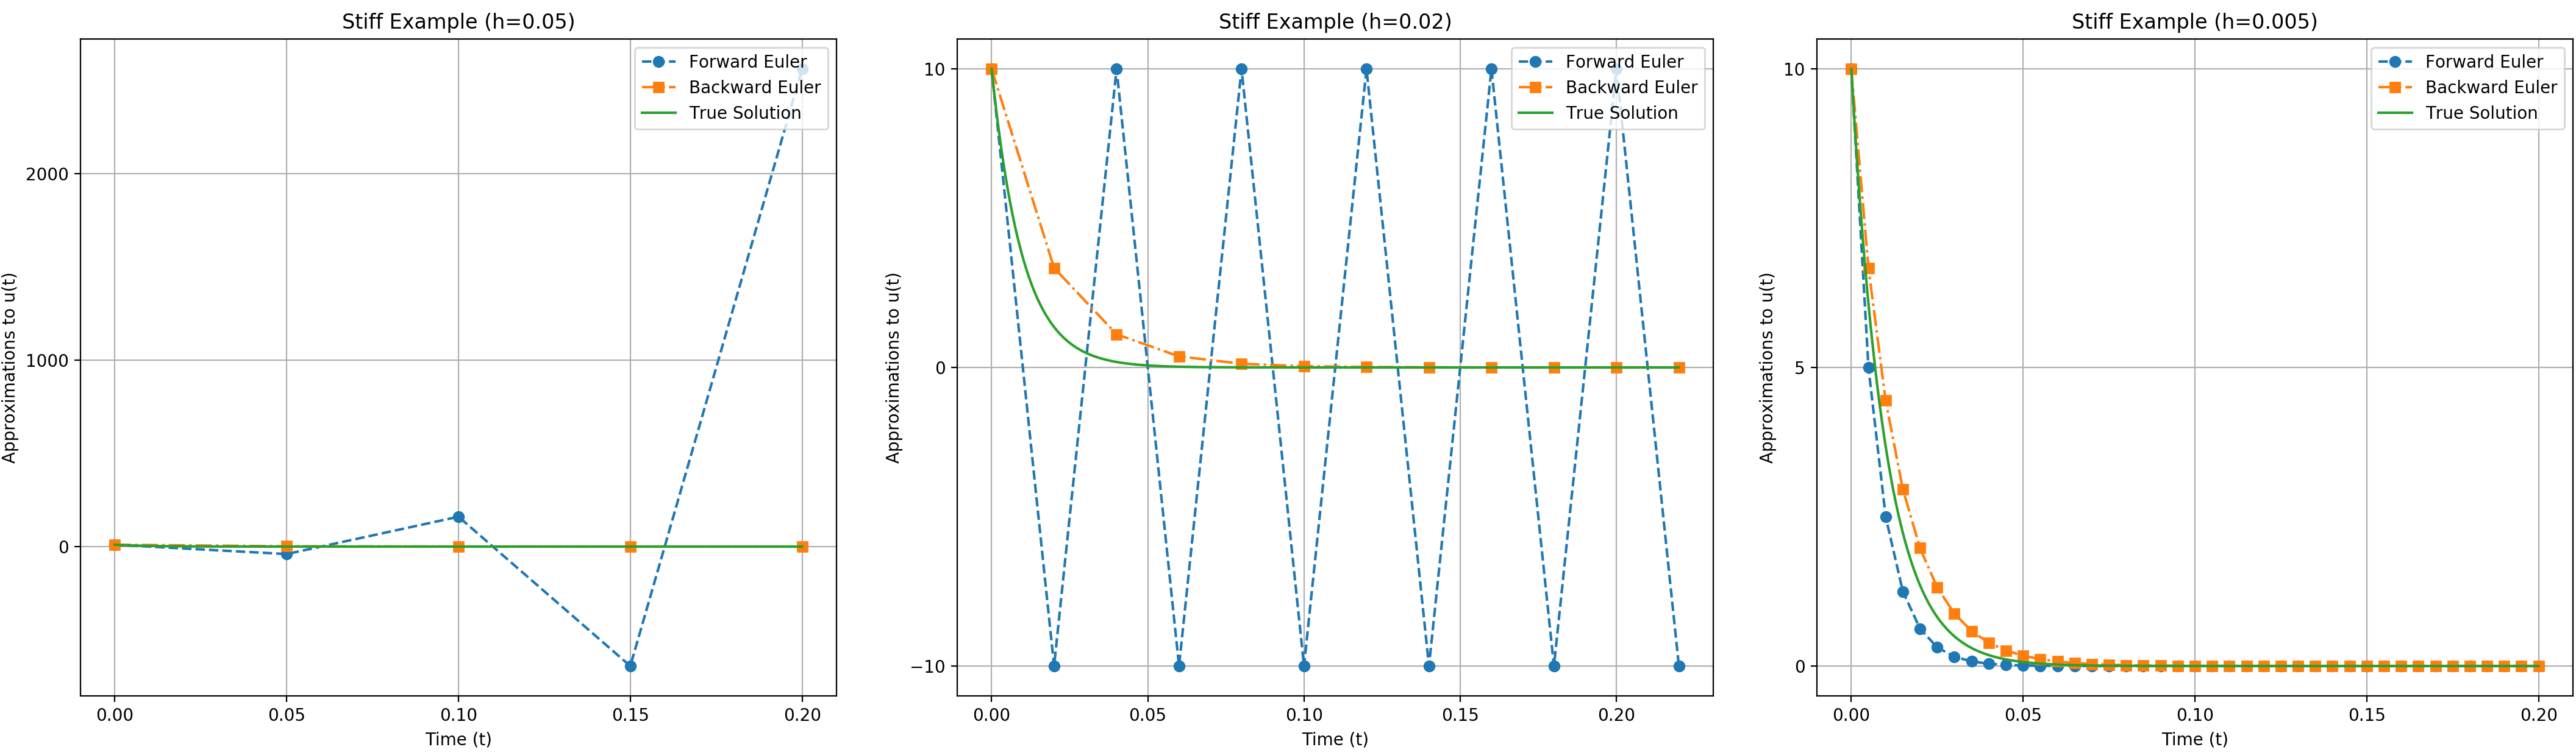
\includegraphics[width=\columnwidth]{stiff_graphs}
                        \caption{Demonstration of stiffness using 
                        \eqref{eq:euler} \& \eqref{eq:backward_euler}
                        with $h=0.05, 0.02, 0.005$ on \eqref{eq:2_stiff_ex}}
                        \label{2_stiff_graphs}
                \end{figure}
            \end{example}

            In summary, we must be careful when choosing numerical methods to 
            solve stiff equations. Depending on the stiffness, we must decide 
            between the performance of choosing an explicit method with 
            smaller steps or using an implicit method with larger steps, but 
            needing to numerically solve an equation such as 
            \eqref{eq:nonlinear_equation} at each iteration.

    \section{Runge-Kutta Methods}
    \label{2_runge_kutta}
        Runge-Kutta methods (first discussed by Runge 1895) look to solve the 
        problem of \textit{improving the accuracy of our approximations 
        without the need to take significantly smaller time intervals?}. Here 
        we won't discuss Runge-Kutta methods in much depth as it is outside of 
        the scope of this project, but we will mention asymptotic complexity 
        and derivations.

        From attempting to integrate \eqref{eq:ivp}, we can apply a Gauss quadrature rule,
        \begin{equation}
        \label{eq:fundamental_theorem_calculus}
            \mathbf{u}_{i+1} = \mathbf{u}_i + \int_{t_i}^{t_{i+1}} 
            \mathbf{u}'(t) dt,
        \end{equation}
        to solve our differential equation. It is with this idea that Runge-Kutta methods were established.

        The general notion is that if we can evaluate intermediate values 
        (or \textit{stages}) between $\mathbf{u}_i$ and $\mathbf{u}_{i+1}$, we can better approximate $\mathbf{u}_{i+1}$. 

        \subsection{4-Stage Runge-Kutta}
        \label{2_rk4}
            Generally the most popular Runge-Kutta method is known as the 
            \textit{Classical Runge-Kutta} which is in fact a special case of 
            the generalised 4-stage Runge-Kutta. The generalised form has $10$
            free parameters, optimising these parameters to yield the highest 
            possible \textit{order} gives us our `Classical' method. This 
            method is given by the iterative scheme,
            \begin{equation}
            \label{eq:rk4}
                \begin{split}
                    \mathbf{u}_{i+1} &= \mathbf{u}_i + 
                    \frac{h}{6} (\mathbf{k}_1 + 2\mathbf{k}_2 + 2\mathbf{k}_3 
                    + \mathbf{k}_4), \quad 
                    \text{where }\\
                    \mathbf{k}_1 &= \mathbf{f}(t_i, \mathbf{u}_i),\\
                    \mathbf{k}_2 &= \mathbf{f}(t_i+\frac{h}{2}, 
                    u_i+\frac{1}{2}\mathbf{k}_1),\\
                    \mathbf{k}_3 &= \mathbf{f}(t_i+\frac{h}{2}, 
                    \mathbf{u}_i+\frac{1}{2}\mathbf{k}_2),\\
                    \mathbf{k}_4 &= \mathbf{f}(t_i+h, 
                    \mathbf{u}_i+\mathbf{k}_3).
                \end{split}
            \end{equation}
            This method is fourth order as $\tau(h)=O(h^5)$. 

            In practice, Runge-Kutta methods have great accuracy properties
            and for small examples often yield sufficient results at a 
            reasonable time cost. Their downsides however, are in the fact
            that every iteration we are computing a number of intermediate
            values and then discarding them at each step. These 
            intermediate function evaluations actually dominate our 
            algorithm's running time. Consequently, when working on large 
            systems of complicated ODEs our computations become very 
            inefficient. 

    \section{Linear Multistep Methods}
    \label{2_lmms}
        In a similar vein to Runge-Kutta methods, Linear Multistep Methods 
        look to use more information from $t<t_{i+1}$ to improve our 
        approximations. In contrast to Runge-Kutta methods, LMMs use 
        previously computed values in their schemes which helps to avoid the problem highlighted at the end of Section \ref{2_runge_kutta}.

        Unlike aforementioned one-step methods, LMMs are not 
        \textit{self-starting} and in order to carry out the first steps, a 
        starting scheme must be decided on. Often a Runge-Kutta method of
        appropriate order is used as a starting routine. This method is chosen
        to have an order equal to or higher than the coupled LMM, to preserve
        asymptotic accuracy.

        \subsection{Adams Methods}
        \label{2_adams}
            Adams methods were devised in the late 19th century (prior to 
            Runge). They are derived from trying to solve the integral 
            equation,
            \begin{equation}
            \label{eq:2_int_equation}
                \mathbf{u}(t_{i+1}) = \mathbf{u}(t_i) + \int_{t_i}^{t_{i+1}}
                \mathbf{f}(t, \mathbf{u}(t)) dt,
            \end{equation}
            by approximating our integrand by a polynomial which interpolates
            our previously computed $\mathbf{u}_j$ values.

            A $k$-step \textit{Adams-Bashforth} method is an \textit{explicit}
            Adams scheme which interpolates to $k$ values to approximate 
            our integrand, $\mathbf{f}(t, \mathbf{u}(t))$. A $k$-step method 
            has LTE of $\tau(h)=O(h^{k+1})$, so is order $k$. It's worth 
            noting that over the bounds of our integral, $(t_i, t_{i+1})$, we 
            are \textit{extrapolating} which is often unreliable.

            The $2$ and $3$-step Adams-Bashforth methods are given by their 
            iterative schemes,
            \begin{align}
                \mathbf{u}_{i+1} &= \mathbf{u}_{i} + \frac{h}{2} 
                (3\mathbf{f}(t_i, \mathbf{u}_i) - 
                \mathbf{f}(t_{i-1},\mathbf{u}_{i-1}))
                \label{2_ab2},\\
                \mathbf{u}_{i+1} &= \mathbf{u}_{i} + \frac{h}{12} 
                (23\mathbf{f}(t_i, \mathbf{u}_i) - 
                16\mathbf{f}(t_{i-1},\mathbf{u}_{i-1}) + 
                5\mathbf{f}(t_{i-2}, \mathbf{u}_{i-2})) \label{2_ab3}.
            \end{align}

            Implicit Adams schemes are known as \textit{Adams-Moulton} 
            methods. They are derived in a similar way to Adams-Bashforth 
            methods except a $k$-step \textit{Adams-Moulton} method looks to 
            approximate the integrand with a polynomial which interpolates to 
            $k+1$ points. This results in integrating over an interpolated 
            region which is much more reliable than the explicit schemes. 

            The trade-off for this increase in stability is that we must solve
            a non-linear equation (similar to \eqref{eq:nonlinear_equation}) at
            every iteration -- which we know is costly.

            The $1$ and $2$-step Adams-Moulton methods are given by their 
            iterative schemes,
            \begin{align}
                \mathbf{u}_{i+1} &= \mathbf{u}_{i} + \frac{h}{2} 
                (\mathbf{f}(t_i, \mathbf{u}_i) + 
                \mathbf{f}(t_{i+1},\mathbf{u}_{i+1})),
                \label{eq:2_am1}\\
                \mathbf{u}_{i+1} &= \mathbf{u}_{i} + \frac{h}{12} 
                (5\mathbf{f}(t_{i+1}, \mathbf{u}_{i+1}) +
                8\mathbf{f}(t_{i},\mathbf{u}_{i}) -
                \mathbf{f}(t_{i-1}, \mathbf{u}_{i-1}))\label{eq:2_am2}.
            \end{align}

            A $k$-step Adams-Moulton method is order $k+1$.


        \subsection{Nystr\"om Methods}
        \label{2_nystrom}
            Similar to Adams, Nystr\"om used the fundamental theorem of 
            calculus to derive an integral equation which could be solved by
            approximating the intergrand. Unlike in \eqref{eq:2_int_equation}, 
            Nystr\"om's integral equation acts over the larger time interval
            $(t_{i-1}, t_{i+1})$. The integral equation is,
            \begin{equation}
            \label{eq:nystrom_int_equation}
                \mathbf{u}(t_{i+1}) = \mathbf{u}(t_{i-1}) 
                + \int_{t_{i-1}}^{t_{i+1}} \mathbf{f}(t, \mathbf{u}(t)) dt.
            \end{equation}

            Nystr\"om methods are \textit{explicit}. In this report we will 
            apply the 2-step \textit{Leapfrog method}, which is defined by the 
            iterative scheme,
            \begin{equation}
            \label{eq:leapfrog}
                \mathbf{u}_{i+1} = \mathbf{u}_{i-1} + 2h\mathbf{f}(t_i, 
                \mathbf{u}_i),
            \end{equation}
            and has order 2.

        \subsection{Backwards Differentiation Formulae}
        \label{2_bdf}
            Unlike Nystr\"om and Adams methods, \textit{Backwards 
            Differentiation Forumlae} (BDF) methods do not look to numerical
            integration for their derivations. Instead, the idea is to 
            start with an interpolating polynomial to directly approximate 
            our solution function. Then, by numerically differentiating our
            interpolant, we substitute this approximation into our IVP and 
            derive our iterative scheme. 

            BDF methods are \textit{implicit} methods, so they come with the 
            same caveats as the Adams-Moulton methods -- that is, the trade off
            between stability and computational cost. BDF methods are 
            \textit{A-stable}, so are appropriate to solve \textit{stiff} 
            equations (popularised by Gear, 1971). 

            The 2-step BDF method (or \textit{BDF-2}) is given by the 
            iterative scheme,
            \begin{equation}
            \label{eq:2_bdf2}
                \mathbf{u}_{i+1} = \frac{4}{3}\mathbf{u}_i - 
                \frac{1}{3}\mathbf{u}_{i-1} + 
                \frac{2h}{3}\mathbf{f}(t_{i+1}, \mathbf{u}_{i+1}),
            \end{equation}
            and is second order.


    \section{Predictor-Corrector Methods}
    \label{2_predictor_correctors}
        Ignoring their computational cost, \textit{implicit} methods are more
        favourable when wanting a one-size-fits-all family of algorithms due 
        to their excellent stability properties. But how do we reduce their
        cost?

        Functional iteration is the natural way that one might attempt to 
        evaluate $\mathbf{u}_{i+1}$ at each step. But this actually creates
        more problems than it solves (especially in stiff equations) and only 
        converges to our solution \textit{linearly}. We have already mentioned
        the use of numerical root finders. Newton's method is a popular choice 
        as on paper it converges quadratically -- yielding a faster convergence 
        for a similar cost. In fact this is not the case. As discussed in 
        \cite{press}, when the Jacobian matrix is approximated via finite 
        differences (as it is in most ODE solvers), Newton's method converges 
        \textit{superlinearly} with an order of convergence $\sqrt{2}$. 
        Predictor-corrector methods avoid these problems and attempt to make 
        good use of the desirable properties of both \textit{explicit} and 
        \textit{implicit} methods.

        \begin{definition}
        \label{2_pc_method}
            A \textbf{predictor-corrector} method is a method pairing with 
            an \textit{explicit} predictor to produce a value 
            $\mathbf{u}_{i+1}^*$ which is substituted into an 
            \textit{implicit} corrector to produce our desired value, 
            $\mathbf{u}_{i+1}$. Predictor-correctors have the form,
            \begin{align}
                \mathbf{u}_{i+1}^* &= \boldsymbol\Phi^* (\text{
                previously computed values of }\mathbf{u}),\\
                \mathbf{u}_{i+1} &= \boldsymbol\Phi(\mathbf u_{i+1}^*, 
                \text{previously computed values of }\mathbf u),
            \end{align}
            where $\boldsymbol\Phi^*, \boldsymbol\Phi $ are chosen explicit 
            and implicit schemes respectively.
        \end{definition}

        There are different variants of predictor-correctors, PEC, PECE and 
        P(EC)\textsuperscript{k}E. These letters refer to the steps carried 
        out in implementation -- \textit{Predict, Evaluate (derivative), 
        Correct, Evaluate (derivative)}. For the purposes of this project, all 
        predictor-correctors followed the PECE structure to simplify 
        implementation.

        It is common for Adams-Bashforth and Adams-Moulton methods to be used
        as a predictor corrector pair. We will also be considering the 
        Forward-Backward Euler, Heun and Leapfrog-BDF2 pairings.


    \section{Adaptive Step-Size}
    \label{2_adaptive}
        Due to Milne, predictor-corrector methods give us an inexpensive way to
        approximate our LTE at each iteration. This error estimate is known as 
        \textit{Milne's device} and is given by,
        \begin{equation}
        \label{eq:2_milnes_device}
            \text{LTE} \approx \frac{C_{p+1}}{C_{p+1} - C_{p+1}^*} 
            (\mathbf{u_{i+1} - u_{i+1}^*}),
        \end{equation}
        where $p$ is the order of our scheme and $C_{p+1}, C_{p+1}^*$ are the 
        error constants for the predictor and corrector respectively). 

        This error estimate allows us to optimise our computations so that when
        our LTE is high we can \textit{decrease} our step-size to reduce our 
        error and \textit{increase} our step size when our LTE is low. We will 
        be adapting our step-size using the formula,
        \begin{equation}
        \label{eq:adapt}
            h_{i+1} = h_i \left(\frac{\text{tol}} 
            {\norm{\text{LTE}}_2}\right)^{\frac{1}{p+1}},
        \end{equation}
        where $\text{tol}$ is some user defined tolerance. 

        When using one-step predictor-corrector pairs, we can go right ahead 
        and apply \eqref{eq:adapt}. Unfortunately, the same cannot be said for 
        LMMs, since in deriving their iterative schemes we have assumed a fixed
        $h$. This leaves two options,
        \begin{enumerate}[label=(\roman*)]
            \item{derive new schemes which account for adaptive $h$, or}
            \item{interpolate backwards to evaluate values of $\mathbf{u}$
            using this step's fixed $h$.}
        \end{enumerate}
        In our implementation, we used (i) by deriving adaptive step schemes
        using Lagrange interpolation (see Appendix ??).


\chapter{Design \& Implementation}
\label{3_implementation}
    \section{Choice of Python}
    \label{3_python}
        The numerical methods discussed in Chapter \ref{2_methods} were 
        implemented in Python primarily due to its \textit{NumPy} package
        and extensive \textit{Matplotlib} graphing capabilities. 

        NumPy provides many optimised vector operations in the box which 
        overload standard binary operations. This allows for flexible code 
        which need not distinguish between vector or scalar operations, 
        helping to maintain a higher-lever approach when programming.

        As mentioned in \ref{2_backward_euler}, we use another python package
        \textit{SciPy} for its modified Powell hybrid method to solve our
        non-linear equations in implicit methods. 

        Clearly, our algorithms would run faster if they were implemented in a
        lower level language such as C/C++, but the focus of the project was to
        investigate the different methods rather than implementing them in the 
        most performant way. 


    \section{Object-Oriented Design}
    \label{3_oo}
        Since our methods have most of the same requirements as each other, an 
        object-oriented approach was chosen to maximise code reuse. In this 
        design, we give each method their own class which is itself the child 
        of some \textit{abstract} class which inherits directly from the 
        \textit{abstract Solver} class. 

        Figure \ref{3_uml} shows a reduced representation of the inheritance
        structure of our different \textit{Solver} classes (where the 
        \mintinline{python}{ForwardEulerSolver} and 
        \mintinline{python}{LeapfrogSolver} are just examples of 
        \mintinline{python}{OneStepSolver} and 
        \mintinline{python}{MultiStepSolver}'s children). 

        \begin{figure}[H]
            \centering
                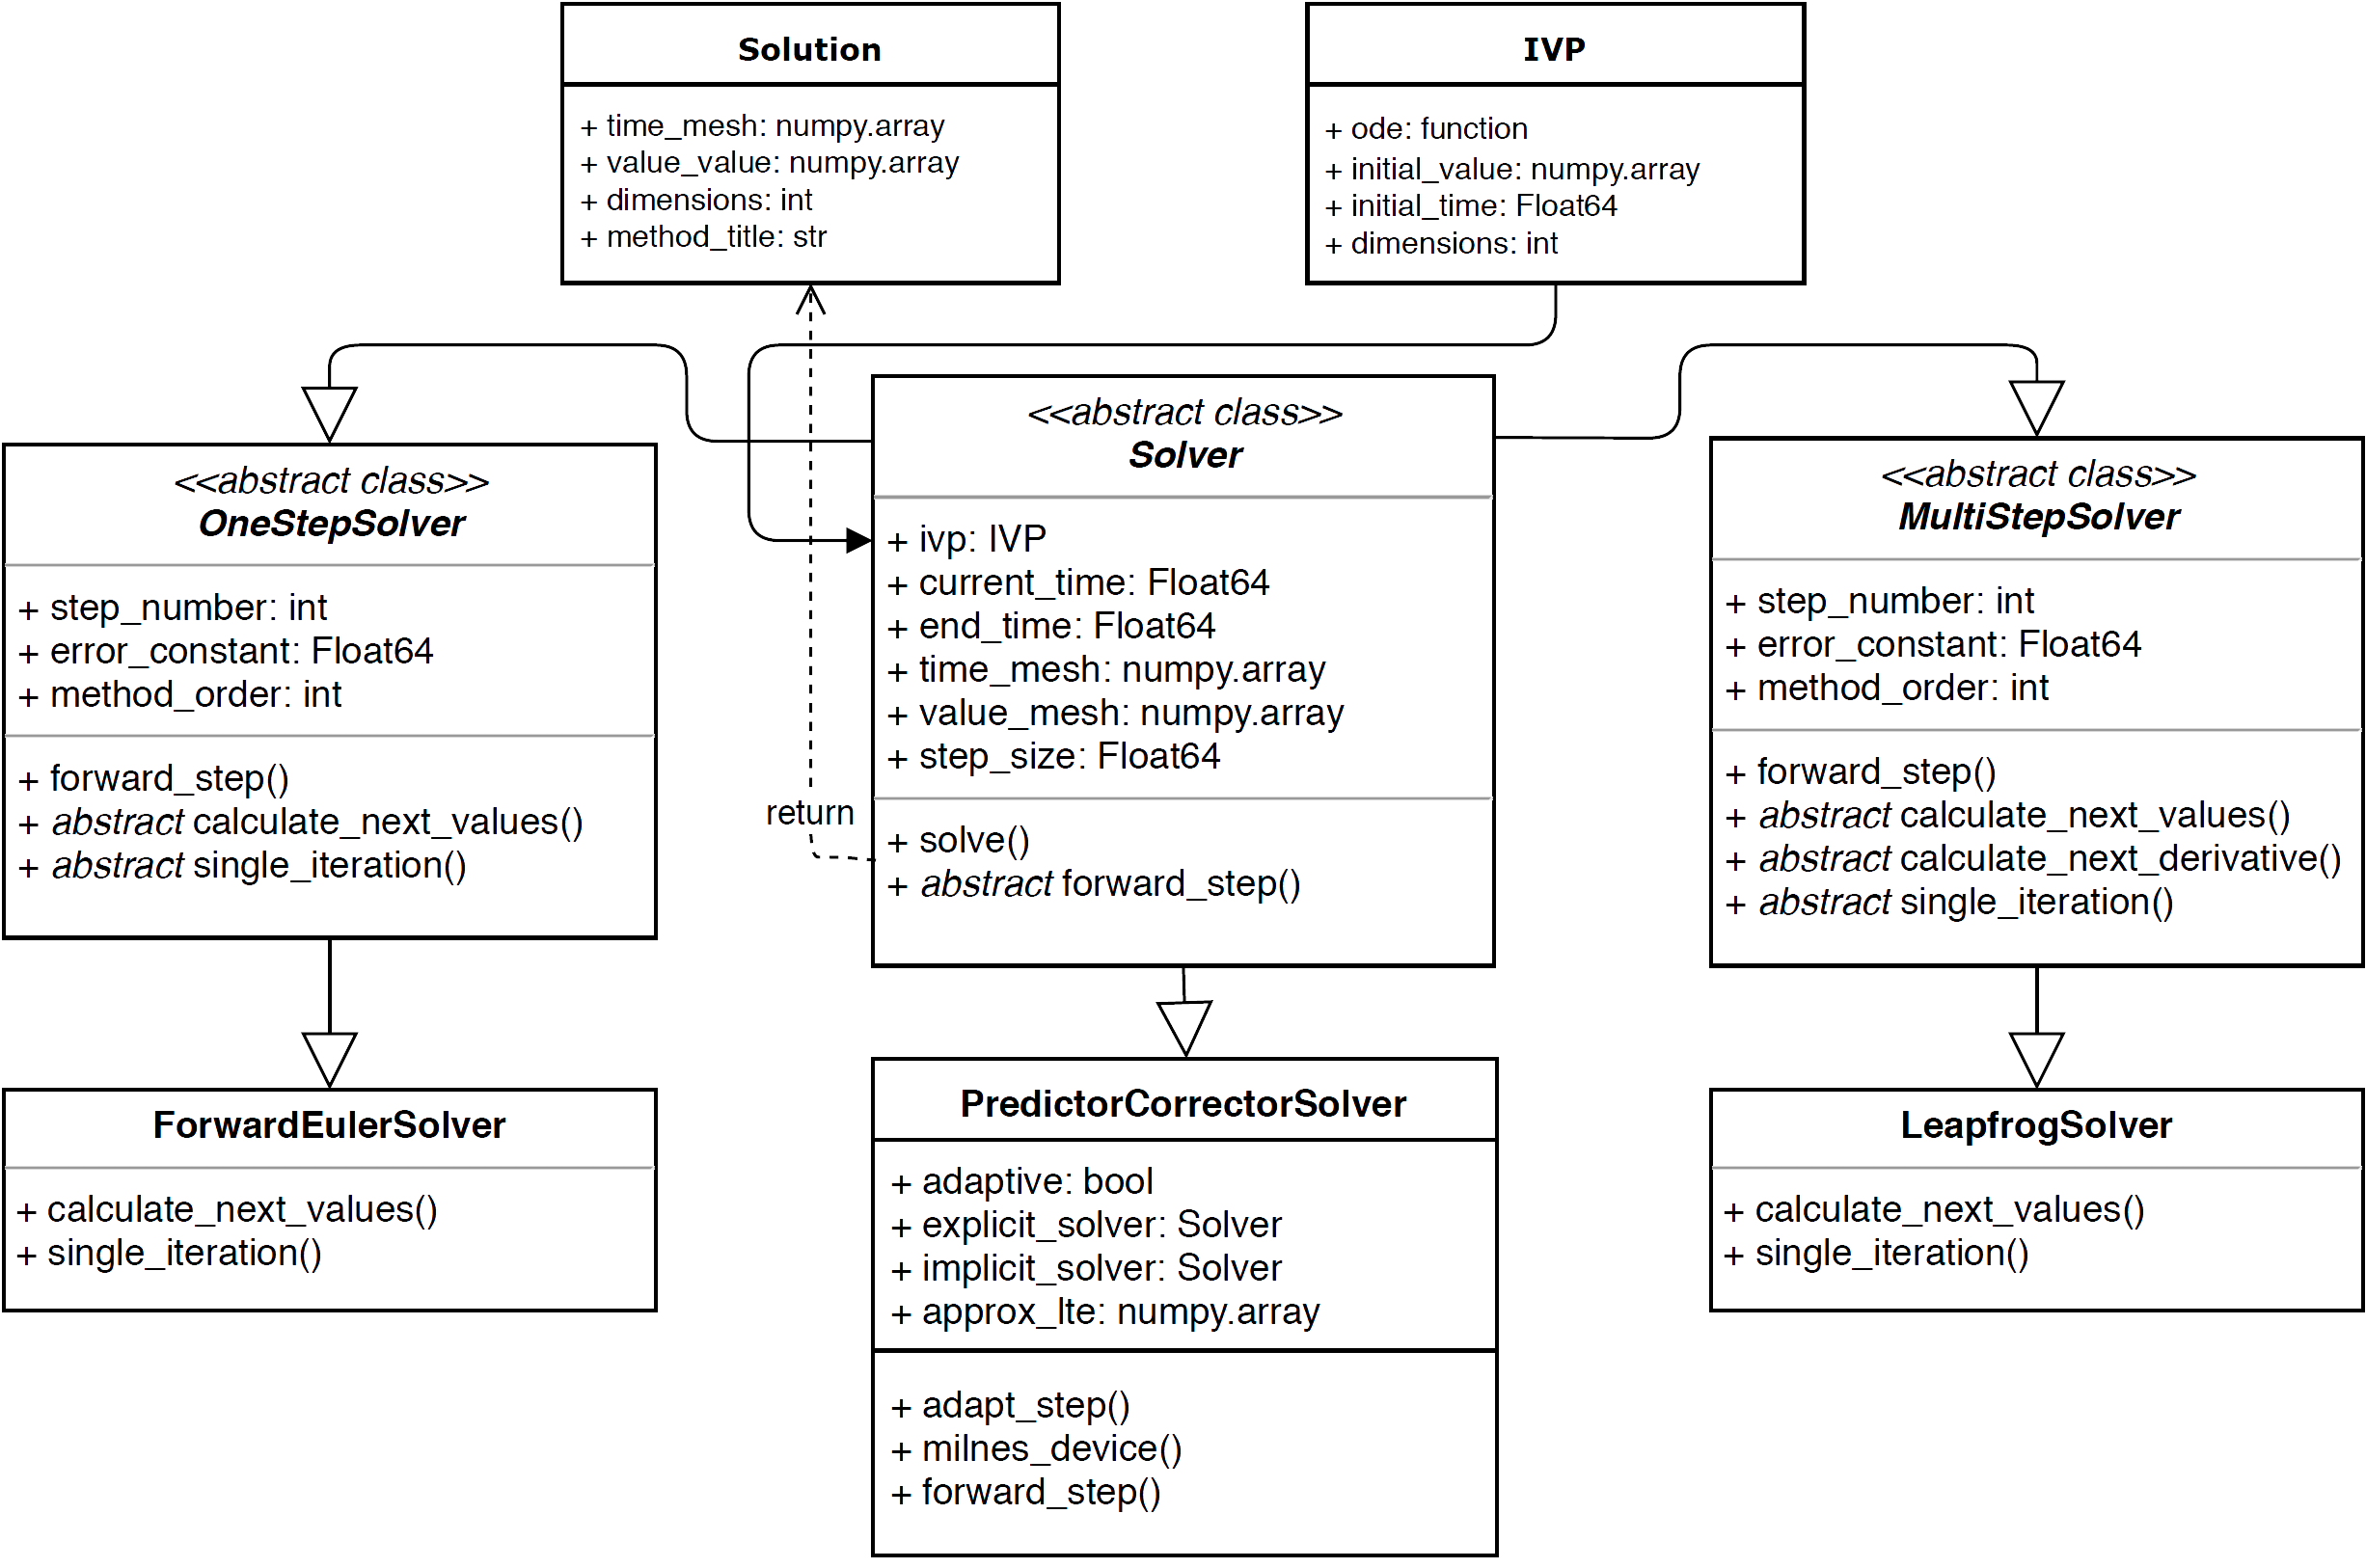
\includegraphics[width=0.9\columnwidth]{uml_diagram}
                \caption{UML diagram of Solver class heirarchy}
                \label{3_uml}
        \end{figure}

        Following Section \ref{2_methods}, we categorised our numerical
        methods into one-step and multi-step methods, which appeared a natural 
        way to split our class definitions. The major difference between
        \mintinline{python}{OneStepSolver} and 
        \mintinline{python}{MultiStepSolver} is that in the latter class we 
        cache our function evaluations between iterations. 

        Aside from predictor-corrector pairs, when comparing two methods we 
        see that they semantically only differ in their iterative scheme 
        (implemented in the \mintinline{python}{calculate_next_values} 
        and\linebreak \mintinline{python}{single_iteration} methods). 
        Therefore all methods share the same \mintinline{python}{solve} which 
        is inherited from our \mintinline{python}{Solver} class. 

        \begin{listing}[H]
            \begin{minted}{python}
                def solve(self):
                    while self.current_time <= self.end_time:
                        self.forward_step(step_counter)

                    self.solution = Solution(self.time_mesh, self.value_mesh)
            \end{minted}
            \caption{
            Outline of \mintinline{python}{solve} method for a \textit{Solver}}
            \label{3_solve}
        \end{listing}
        
        Since our \textit{Solver} classes have numerous `helper' instance 
        variables the decision was made to produce a (lighter weight) 
        \mintinline{python}{Solution} object which contains only the matrix of
        results and time mesh. This allowed for a simpler reporting process
        when wanting to graph results.

        \mintinline{python}{OneStepSolver} and 
        \mintinline{python}{MultiStepSolver} have
        \mintinline{python}{forward_step} methods of the form,
        \begin{listing}[H]
            \begin{minted}{python}
                def forward_step(self, step):
                    # next_step_size is class property, so it can vary between steps
                    this_h = self.next_step_size
                    self.time_mesh[step] = self.time_mesh[step - 1] + this_h
                    self.value_mesh[step] = self.calculate_next_values(step, this_h)
                    self.derivative_mesh[step] = self.calculate_next_derivative(step)
            \end{minted}
            \caption{Outline of \mintinline{python}{forward_step} method for 
                     a \textit{Solver}}
            \label{3_forward_step}
        \end{listing}
        \noindent where the \mintinline{python}{OneStepMethod} class omits 
        line 6.

        Since Multi-step methods are not self starting,
        \mintinline{python}{MultiStepSolver} objects are coupled with a 
        \mintinline{python}{OneStepSolver} object when they are instantiated. 
        If otherwise unspecified, the \textit{Classical Runge-Kutta} method 
        \eqref{eq:rk4} is used.



        \subsection{Predictor-Corrector Implementation}
            Prior to the implementation of the predictor-corrector, standalone 
            algorithms operated on the basis of calling their
            \mintinline{python}{solve} method which, in turn, iteratively calls
            instance methods, mutating the state of our \textit{solver} 
            object. Calling methods to update instance variables is set out by
            our \mintinline{python}{Solver} class.

            Given that predictor-correctors are themselves \textit{solvers}, 
            our class representation should reflect this. So 
            \mintinline{python}{PredictorCorrectorSolver} is a 
            child class of \mintinline{python}{Solver} (as shown in 
            \ref{3_uml}). This means that the predictor-corrector has its own 
            state. 

            Definition \ref{2_pc_method} tells us that a predictor-corrector
            is made up of an \textit{explicit-implicit} pair. It was decided 
            that when constructing a 
            \mintinline{python}{PredictorCorrectorSolver} object we 
            pass it explicit and implicit solver objects which share the same
            \mintinline{python}{ivp} attribute. One issue which arises from 
            this design is that of \textit{ownership}. Since we are interested
            in the predictor-corrector \textit{pair}, we want to ensure that we
            are updating the \mintinline{python}{PredictorCorrectorSolver}'s 
            state at each time step accordingly. We acheive this by giving all
            solvers a static method \mintinline{python}{single_iteration} which
            emulates the behaviour of the existing 
            \mintinline{python}{compute_next_values} method. The fundamental 
            difference between these methods is that in 
            \mintinline{python}{single_iteration} we represent our current
            state by passing method arguments and returning values--rather than
            updating instance variables (like in 
            \mintinline{python}{compute_next_values}). Figure \ref{3_pc_uml} 
            briefly outlines these interactions.

            \begin{figure}
                \centering
                    \includegraphics[width=0.6\columnwidth]{%
                    predictor-corrector}
                    \caption{UML diagram showing how 
                    \mintinline{python}{PredictorCorrectorSolver} interacts 
                    with its explicit (e.g. Leapfrog) and implicit 
                    (e.g. Trapezoidal) objects}
                    \label{3_pc_uml}
            \end{figure}

            These method calls all happen inside the 
            \mintinline{python}{forward_step} method in a PECE manner 
            (\ref{2_predictor_correctors}). The outline of the
            \mintinline{python}{forward_step} method is shown in Listing 
            \ref{3_pece}.
            \begin{listing}[H]
                \begin{minted}{python}
                    def forward_step(self, step):
                        self.current_time = self.time_mesh[step] \
                                          = self.time_mesh[step - 1] + self.next_step_size
                        # P: Prediction
                        prediction = self.explicit_solver.single_iteration(self.value_mesh,
                                                                           self.time_mesh,
                                                                           step,
                                                                           self.derivative_mesh)
                        # E: Evaluation
                        derivative = self.ivp.ode.function(prediction, self.current_time)
                        self.update_current_state(step_counter, prediction, derivative)
                        # C: Correction
                        correction = self.implicit_solver.single_iteration(self.value_mesh,
                                                                           self.time_mesh,
                                                                           step,
                                                                           self.derivative_mesh)
                        # E: Evaluation
                        derivative = self.ivp.ode.function(correction, self.current_time)
                        self.update_current_state(step_counter, correction, derivative, lte_approx)
                \end{minted}
                \caption{Outline of 
                \mintinline{python}{PredictorCorrectorSolver.forward_step}}
                \label{3_pece}
            \end{listing}

        \subsection{Adaptive Step-Size Implementation}
        \label{3_adaptive}
            To allow for adaptive step-sizes, \textit{Milne's Device} was used
            to estimate our LTE from a given prediction-correction pair and was
            implemented in \mintinline{python}{milnes_device}. We can append
            Listing \ref{3_pece} with
            \begin{listing}[H]
                \begin{minted}[firstnumber=20]{python}
                    lte_approx = self.milnes_device(prediction, correction)
                    if self.adaptive:
                        self.step_size = self.adapt_step(self.step_size, lte_approx, self.step_tol)
                \end{minted}
                \caption{Adaptive Step snippet from 
                \mintinline{python}{PredictorCorrectorSolver.forward_step}}
                \label{3_adaptive_forward}
            \end{listing}
            \noindent to enable adaptive step computations. The 
            \mintinline{python}{adapt_step} method uses \eqref{eq:adapt} to
            adjust the step size. This method also accomodates for catastrophic
            floating point cancellation and ensures that step sizes are not 
            increased by more than double their previous value.

    \section{Graphs \& Case Study Animations}
    \label{3_case_studies}
        It was important to ensure that results from computations could be 
        graphed and reported on in the same way. This would enable coherent
        and reliable comparisons between methods' behaviours. 

        For both the n-body problem and the double pendulum, animations were 
        produced to help analyse the results of our computations. In both cases,
        existing solutions (\cite{multicomet} \& \cite{pendulum}) where adapted
        to better suit our case studies.

        The n-body animation uses a modification of the built-in 
        \mintinline{python}{comet} function in MATLAB. Bodies were represented
        as point masses (as in Newton's Law of Gravition) and their displayed
        sizes are not representative of the situation we are trying to model.
        The pendulum and double pendulum animations are built directly from an 
        online example in the documentation of the 
        \mintinline{python}{matplotlib} package.

        One added complexity with our animations was that when using variable
        step results not all computed values could be used in animations due to
        the memory load of doing so. For the purposes of animation this is
        unimportant as their main purpose is to provide qualitative feedback on
        the case study. This, however, does highlight a small flaw in the 
        current implementation of our \textit{solvers}. As the number of 
        iterations increase, we are putting much more load on the program's 
        memory. The obvious solution to this would be to write results to disk
        when we no longer require them. It was decided that the details of data
        storage was unimportant for this project, so the initial approach 
        was kept.


\chapter{Comparison of Methods}
\label{4_comparison}
    
    \section{Fixed Step-Size Methods}
    \label{4_fixed}
        Before diving deeper into analysing our predictor-corrector methods, it
        is important to first compare the standalone methods which will later
        make up our predictor-corrector pairs. We will be examining the 
        running time, error accumulation and stability of our algorithms using 
        IVPs with known analytical solutions.

        \begin{example}
        \label{4_example_1}
            Consider the IVP,
            \begin{equation}
            \label{eq:4_ex_1}
                \begin{cases}
                    u'(t) = -\pi \sin(\pi t) + \pi \cos(2\pi t), \quad 
                    \text{on } t \in [0,4],\\
                    u(0) = 1,
                \end{cases}
            \end{equation}
            whose analytic solution is given by $u(t)=\cos(\pi t)+ 
            \frac{1}{2}\sin(2\pi t)$. Solutions to this IVP were computed
            using the explicit solvers, \textit{Forward Euler} \eqref{eq:euler},
            \textit{Adams-Bashforth 2-Step} \eqref{eq:ab2}, \textit{Leapfrog}
            \eqref{eq:leapfrog}, and the implicit solvers, 
            \textit{Backward Euler} \eqref{eq:backward_euler}, 
            \textit{Trapezoidal} \eqref{eq:am1}, \textit{BDF-2} 
            \eqref{eq:2_bdf2}. Figure \ref{4_graphs_1} shows us these results
            along with their subsequent errors. 
        \end{example}
        \begin{figure}[H]
            \centering
                \includegraphics[width=\columnwidth]{%
                1}
                \caption{Numerical results for Example \ref{4_example_1}
                using a fixed step size $h=0.08$.}
                \label{4_graphs_1}
        \end{figure}

        We can see that both our Forward and Backward Euler methods are 
        significantly less accurate than our other order 2 methods. Since our 
        IVP is non-stiff, it is unsurprising to see that there is very little
        overall difference between the errors in our explicit and implicit 
        schemes. These computations were repeated 1000 times and the 
        running-time of each algorithm's \mintinline{python}{solve} method 
        was logged, producing a mean running-time for each scheme. 
        \begin{table}
            \centering
                \begin{tabular}[H]{| l | l |}
                    \hline
                    Algorithm & Time /$\mu$s \\ \hline
                    Forward Euler & 331 \\ \hline
                    Adams-Bashforth 2-Step & 601 \\ \hline
                    Leapfrog & 407 \\ \hline
                    Backward Euler & 3036 \\ \hline
                    Trapezoidal & 3627 \\ \hline
                    BDF-2 & 5567 \\
                    \hline
                \end{tabular}
                \caption{Running-times of algorithms in Example 
                \ref{4_example_1}.}
                \label{4_1_runtimes}
        \end{table}
        Table \ref{4_1_runtimes} shows that our implicit methods are running
        approximately ten times slower than our explicit ones. Therefore due 
        to Example \ref{4_example_1}'s lack of stiffness an explicit method
        would allow us to minimise cost without sacrificing accuracy. 
        
        We could also apply some predictor-corrector pairs to the IVP
        which would make improvements to the running-time of our implicit 
        schemes in addition to improving their explicit-part's stability 
        properties. The results of doing this are shown in Figure 
        \ref{4_pc_graphs_1}. These results in addition to the figures shown
        in Table \ref{4_pc_runtimes} help to highlight that 
        predictor-corrector methods are an excellent way to maintain or even
        increase accuracy without sacrifising much running-time.
        \begin{figure}[H]
            \centering
                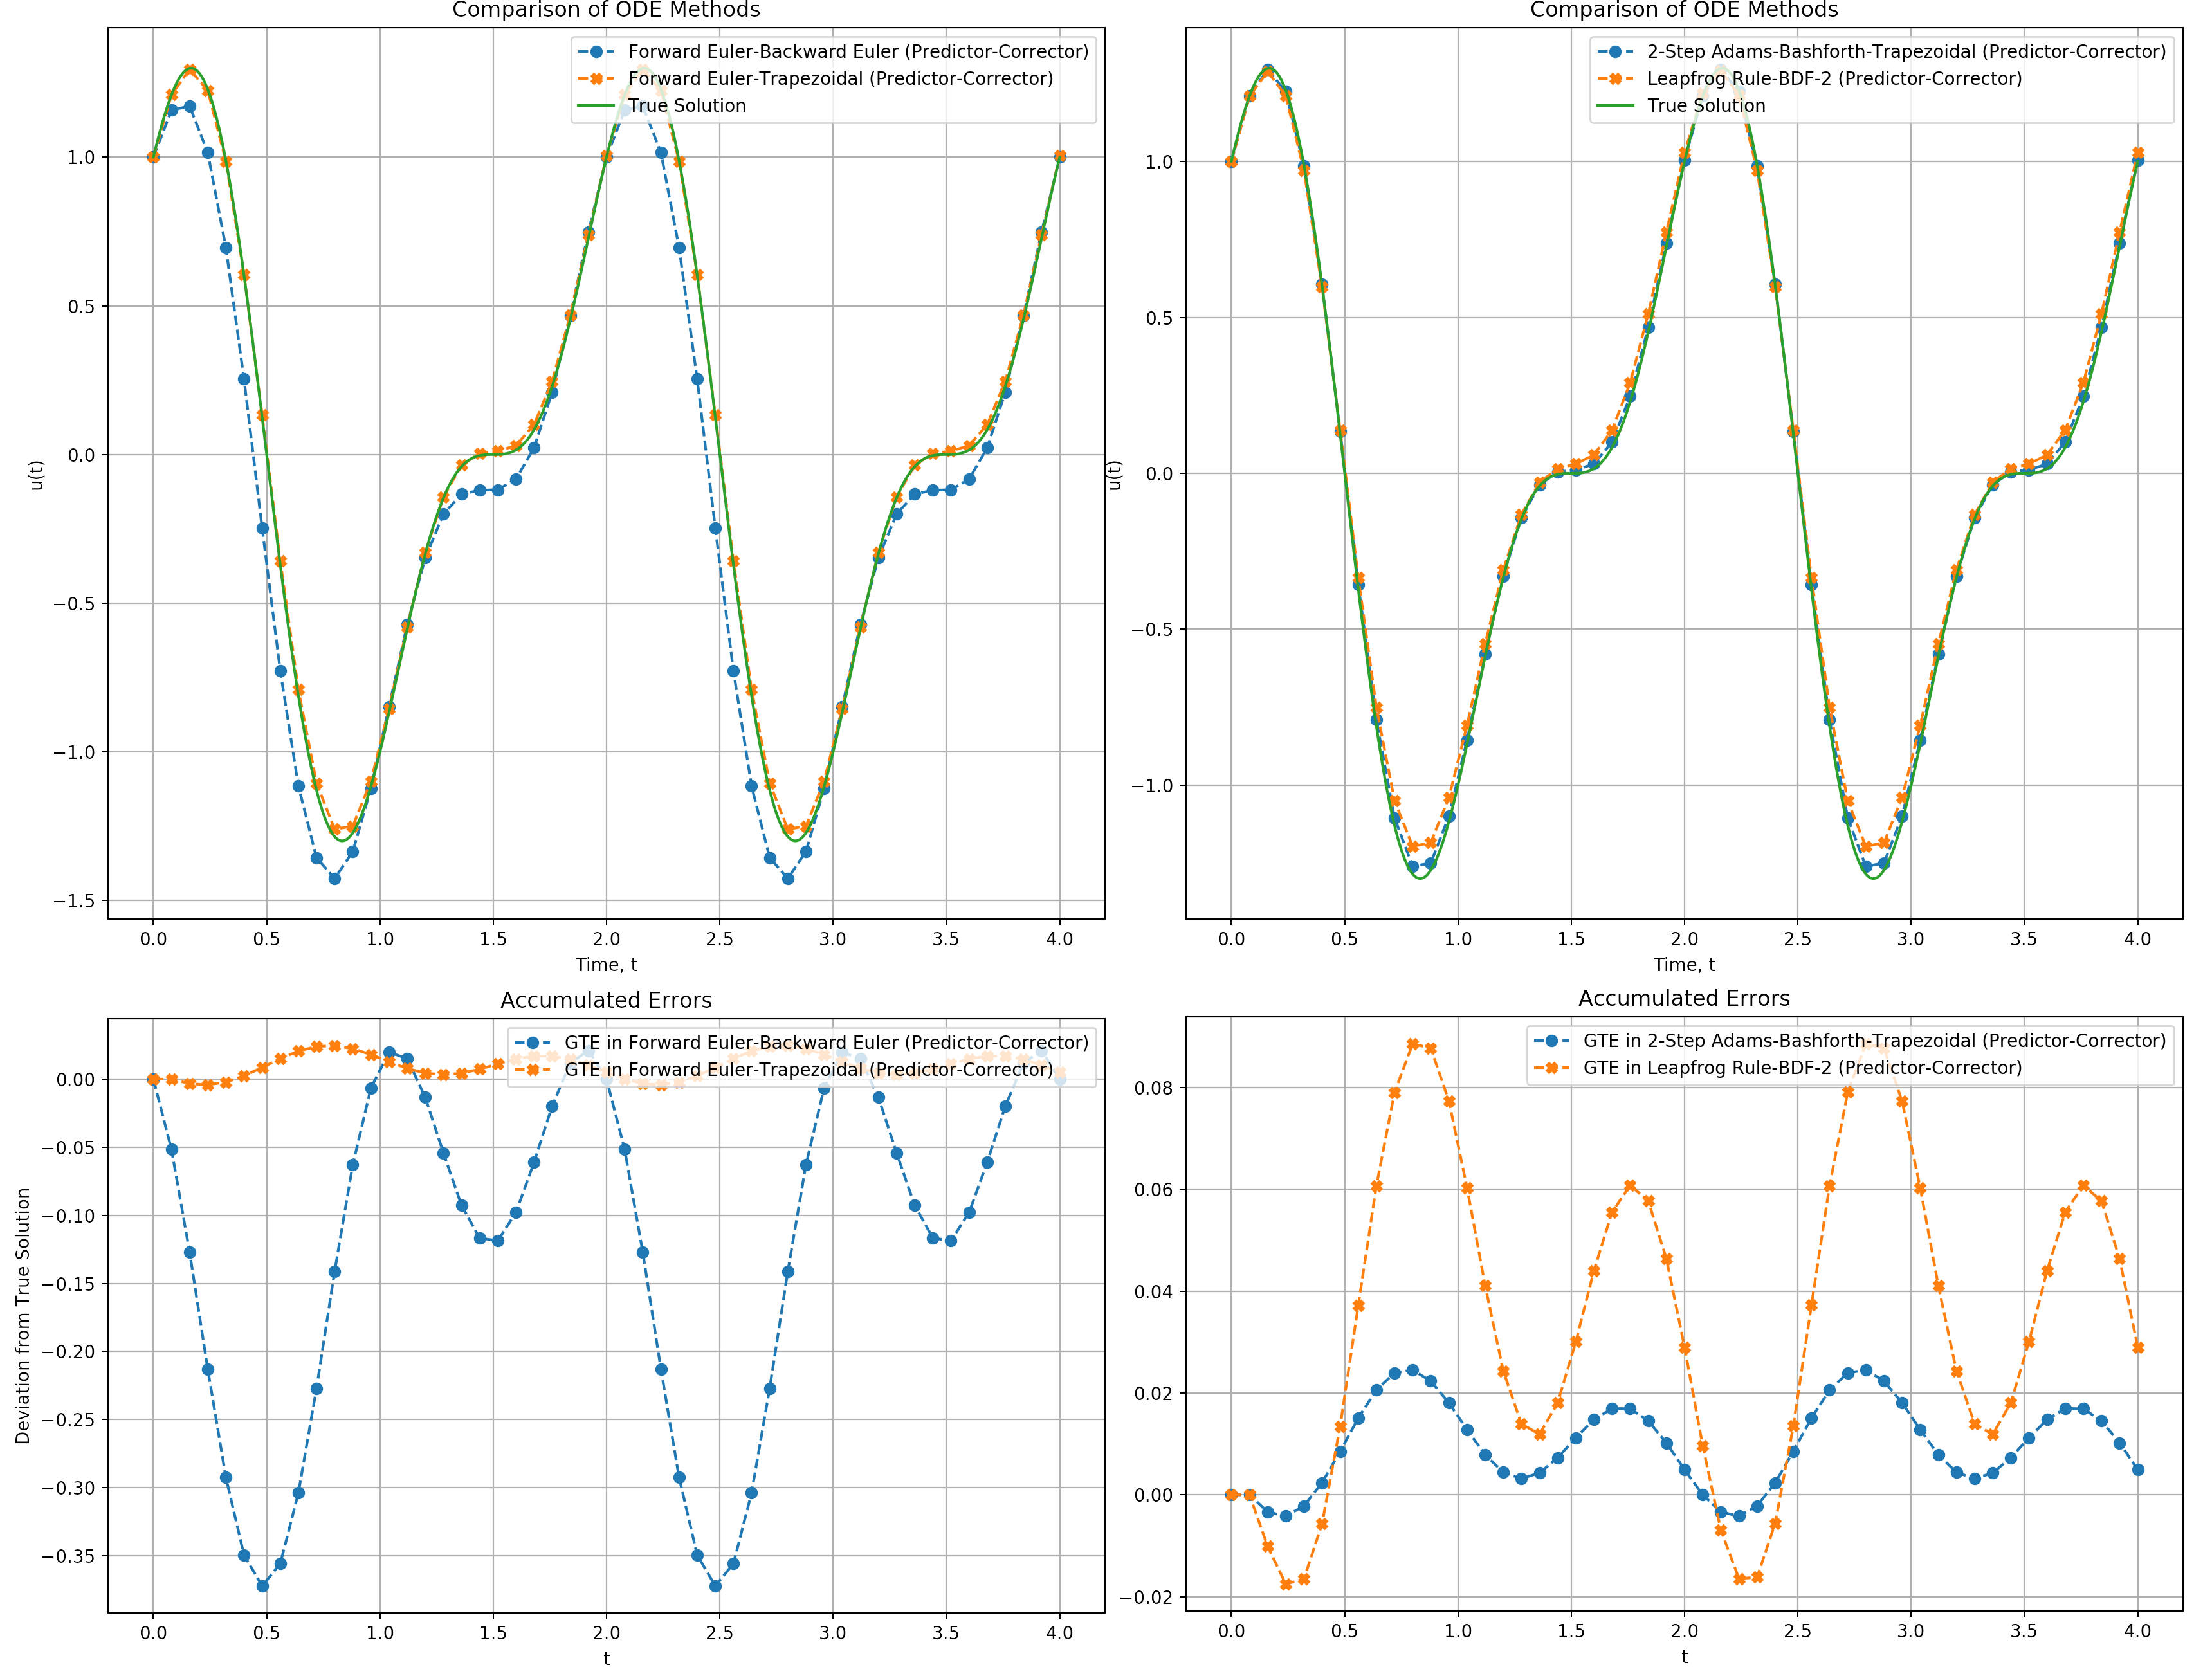
\includegraphics[width=\columnwidth]{1_pc}
                \caption{Numerical results for Example \ref{4_example_1}
                using Predictor-Corrector methods with fixed $h=0.08$.}
                \label{4_pc_graphs_1}
        \end{figure}

        \begin{table}
            \centering
                \begin{tabular}[H]{| l | l | l |}
                    \hline
                    Predictor & Corrector & Time /$\mu$s \\ \hline
                    Forward Euler & Backward Euler & 936 \\ \hline
                    Forward Euler & Trapezoidal & 1061 \\ \hline
                    Adams-Bashforth 2-Step & Trapezoidal & 1211 \\ \hline
                    Leapfrog & BDF-2 & 1297 \\
                    \hline
                \end{tabular}
            \label{4_pc_runtimes}
            \caption{Running-times of Predictor-Corrector pairings in Example
            \ref{4_example_1}.}
        \end{table}

        \begin{example}
        \label{4_example_2}
            Consider the IVP,
            \begin{equation}
            \label{eq:4_ex_2}
                \begin{cases}
                    u'(t) + u(t) = 50\sin (t), \quad 
                    \text{on } t \in [0,1/2],\\
                    u(0) = 1,
                \end{cases}
            \end{equation}
            whose analytic solution is given by 
            \begin{equation}
            \label{eq:4_ex_sol_2}
                u(t) = \frac{1}{2501} \left( 2551e^{-50t} + 2500\sin(t)
                - 50\cos(t)  \right).
            \end{equation}

            Here we look to compare the results of some \textit{implicit} 
            solvers on this stiff equation with those produced from some
            \textit{predictor-corrector} pairs. The results from our 
            computations are shown in Figure \ref{4_ex_2_graphs}.          
        \end{example}
        
        \begin{figure}[H]
            \centering
                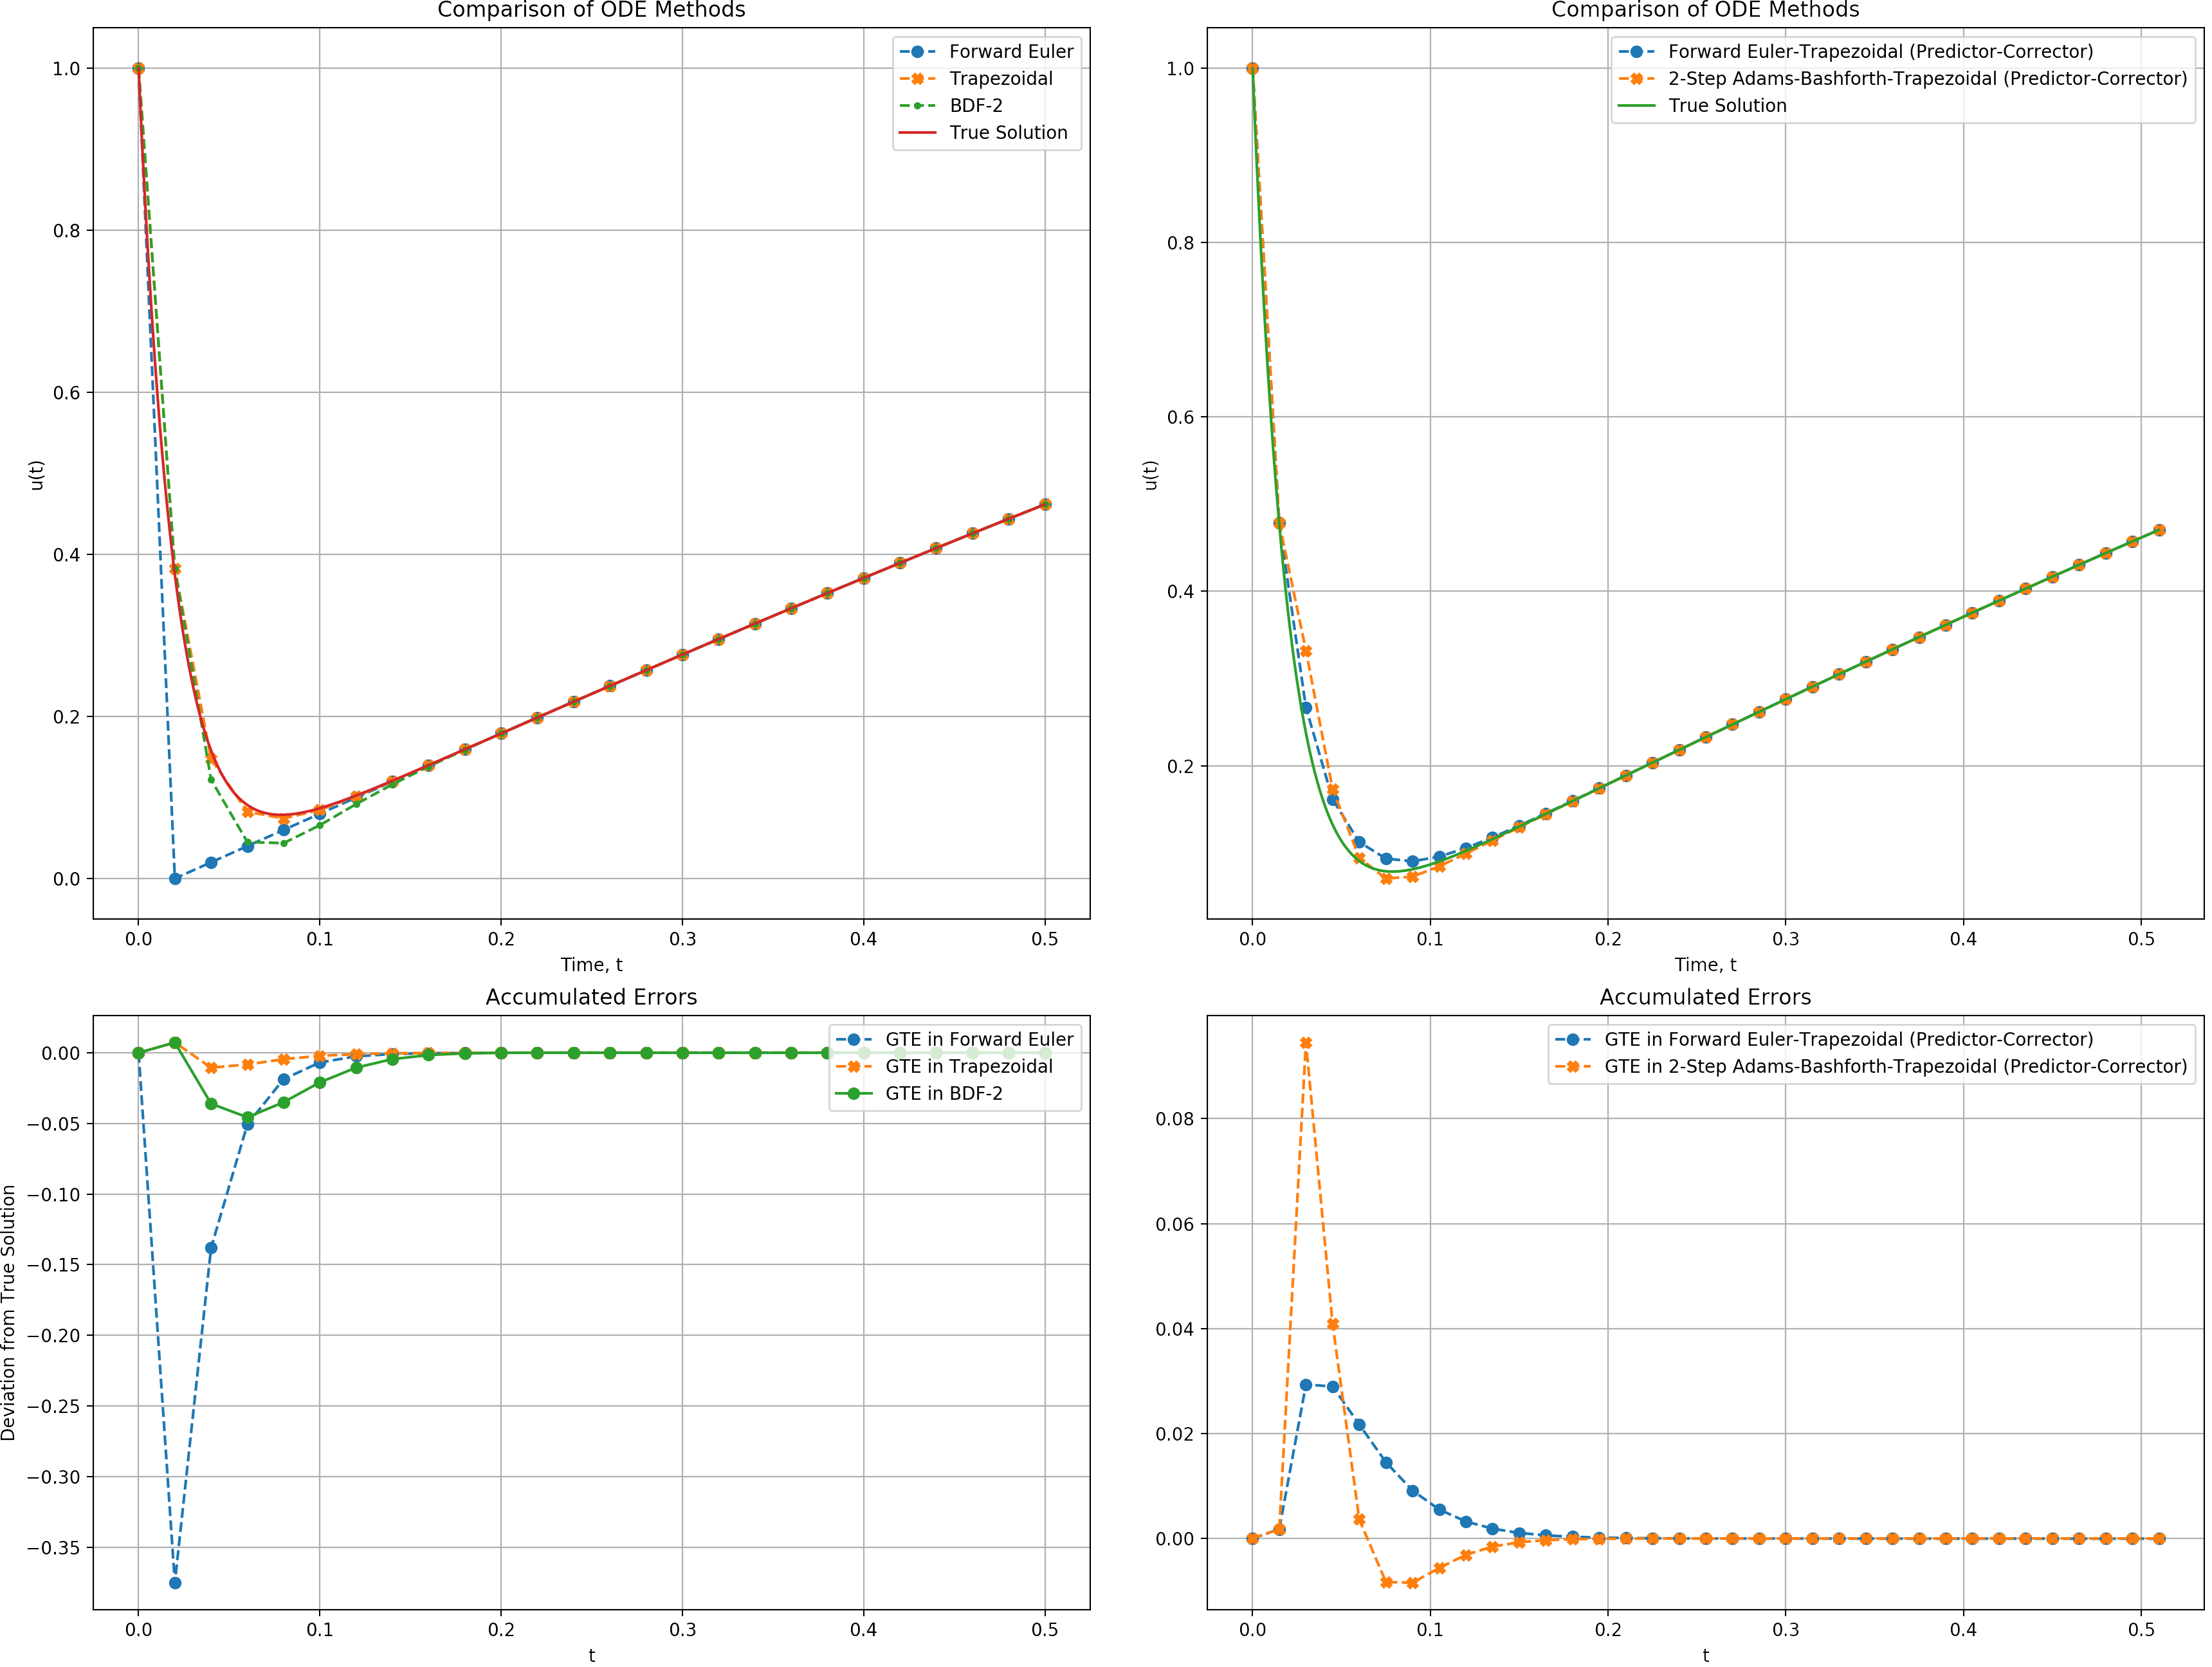
\includegraphics[width=\columnwidth]{2}
                \caption{Numerical results from Example \ref{4_example_2} using
                Implicit and Predictor-Corrector methods with a fixed 
                $h=\num{20e-3}$.}
                \label{4_ex_2_graphs}
        \end{figure}

        This example was chosen due to its \textit{local} stiffness in the 
        range $(0.0, 0.1)$ which, although not dominating at a step-size of 
        $h=\num{20e-3}$, in explicit solvers the characteristics of the solution
        curve would not well be shown at this step size. In fact, we can see that
        when Forward Euler is applied at this $h$ our solution drops in one step
        to ${\sim}0$ and then increases in a psuedo-linear fashion advancing in an
        opposite direction to that of the true solution curve. 

        \begin{table}
            \centering
                \begin{tabular}[H]{| l | l |}
                    \hline
                    Algorithm & Time /$\mu$s \\ \hline
                    Trapezoidal & 2101 \\ \hline
                    BDF-2 & 2613 \\ \hline
                    Forward Euler--Trapezoidal (Heun's) & 969 \\ \hline
                    Adams-Bashforth 2-Step--Trapezoidal & 1074 \\
                    \hline
                \end{tabular}
            \label{4_im_pc_runtimes}
            \caption{Running-times of Predictor-Corrector pairings in Example
            \ref{4_example_2}.}
        \end{table}

    \section{Adaptive Step-Size Methods}
    \label{4_adaptive}
        Practically speaking, this increase in stability is in fact 
        significantly small and is really just an increase in accuracy. Chase
        discusses in \cite{chase} how the stability of a predictor-corrector
        is dominated by the predictor equation. With this in mind, it is 
        clear that the most valuable characteristic of the predictor-corrector
        methods discussed is our ability to inexpensively estimate our LTE
        and therefore adapt our step size to keep errors below a given 
        tolerance. Although this does not provide the most suitable of solvers
        for stiff equations, it does at least mean that errors can somewhat 
        automatically be kept at bay by decreasing the step-size. Also, we can
        increase our step-size to avoid unnecessarily short steps when LTE is 
        low.

        
        
    
\chapter{Case Studies}
\label{5_case_studies}
    \section{$n$-Body Problem}
    \label{5_nbody}

    \section{Pendula}
    \label{pendula}

\chapter{Reflection}
\label{6_reflection}




\clearpage
\section{Deriving the Adaptive 2-step Adams-Bashforth Method}
    \begin{equation}
        e=mc^2
    \end{equation}



\begin{thebibliography}{50}
    \bibitem{ascher}
        U.M.~Ascher, L.R.~Petzold,
        ``Computer Methods for Ordinary Differential Equations and 
        Differential-Algebraic Equations'',
        Philadelphia: SIAM (1935).

    \bibitem{newton}
        I.~Newton,
        ``Philosophiae Naturalis Principia Mathematica (“Mathematical
        Principles of Natural Philosophy”)'',
        London (1687).

    \bibitem{hairer}
        E.~Hairer, S.P.~N{\o}rsett, G.~Wanner,
        ``Solving Ordinary Differential Equations I'',
        Springer-Verlag Berlin Heidelberg (1993).

    \bibitem{higham}
        D.F.~Griffiths, D.J.~Higham,
        ``Numerical Methods for Ordinary Differential Equations'',
        Springer-Verlag London Limited (2010).

    \bibitem{powell}
        ``https://www.math.utah.edu/software/minpack/minpack/hybrd1.html'', 
        ``Documentation for MINPACK subroutine HYBRD1'',
        April 2019.

    \bibitem{suli}
        E.~Suli, D.~Mayers,
        ``An Introduction to Numerical Analysis'',
        Cambridge University Press (2003).

    \bibitem{gregory}
        R.D.~Gregory,
        ``Classical Mechanics'',
        Cambridge University Press (2006).

    \bibitem{press}
        W.T.~Vetterling, W.H.~Press,
        ``Numerical Recipes in C: the art of scientific computing (2nd 
        Edition)'',
        Cambridge University Press (1992).

    \bibitem{pras}
        ``http://www.cs.ox.ac.uk/people/pras.pathmanathan/nmood\_printable.pdf'',
        ``Numerical methods and object-oriented design'',
        January 2019.

    \bibitem{iserles}
        A.~Iserles,
        ``A First Course in the Numerical Analysis of Differential Equations'',
        Cambridge University Press (1996).

    \bibitem{multicomet}
        ``https://uk.mathworks.com/matlabcentral/fileexchange/67945-multicometfade'',
        ``Multiple MATLAB comet trajectory plots'',
        February 2019.

    \bibitem{pendulum}
        ``https://matplotlib.org/gallery/animation/double\_pendulum\_sgskip.html'',
        ``Double Pendulum matplotlib.animation example'',
        March 2019.

    \bibitem{chase}
        P.E.~Chase
        ``Stability Properties of Predictor-Corrector Methods for Ordinary 
        Differential Equations'',
        Journal of the ACM, p.457-468, October 1962

\end{thebibliography}
\end{document}

